%!TEX root = cscw2019-comic.tex
\section{Model Criticism}
% \section{Model Criticism}
\label{sec:Model Criticism}

In this section, we  begin with a short section explaining our choice to use Bayesian analysis. Then in~\ref{sub:Posterior Checks, Convergence and Normality}, we examine model convergence and Normality.

% how well the proposed models explain the observed data, including model convergence.

\subsection{Why Bayesian?}
\label{sub:Why Bayesian?}
In a recent paper,~\textcite{Kay2016}, make a persuasive argument that Bayesian methods are better suited to the HCI community, including making the case that Bayesian methods allow for replicating the results and improving the strength of the conclusions by using previous outcomes as priors. We would add two reasons, in addition to those by~\textcite{Kay2016} to explain our decision to use Bayesian models. 
\begin{description}
    \item[Transparency:] With a Bayesian model, the researcher foregrounds all the aspects of the model; there are no modeling assumptions that need checking, not already foregrounded in the model description. Non-Bayesian statistics are powerful tools, and when used by an experienced statistician, they can dramatically reduce the process of inference. However, for researchers who wish to investigate their findings without access to a statistician, they need to be careful of the assumptions of the different tests: Normality ($t$-test); heteroscedasticity (e.g., ANOVA) and ensuring that the data satisfy the assumptions. Omitting the right sequence of analysis can lead to inferences not supported by the data.
    \item[Small $n$ studies:] A Bayesian model is valid at \textit{every} value of $n$; we do not have to wait for $n\geq 30$ to satisfy assumptions of say Normality. For small $n$ values, the result is of course affected by the choice of the prior; but by using weakly informative priors, we can ensure that the prior doesn't dominate inference. Furthermore, when Bayesian models use maximum entropy likelihood functions (e.g., members of the exponential family, that include the Normal distribution and the gamma distribution), we make the \textit{most conservative} inference given the data. See~\textcite[][Chapter 9]{McElreath2015} for an excellent description of the use of maximum entropy models in Bayesian analysis.
\end{description}


\subsection{Model Convergence and Normality}
\label{sub:Posterior Checks, Convergence and Normality}

\hs{In this section, we examine model convergence and our assumptions about Normality.}

The model shows good convergence, as evidenced by the traceplot in~\Cref{fig:traceplot}. The Gelman-Rubin statistic $\hat{R}$ was around 1, indicating that the different sampling chains converged. Furthermore, the effective sample size of all parameters was greater than 10,000.

\hs{We used the $t$-distribution to model likelihood motivated by the high contributions at \$0 and \$5 in the data (c.f.~\Cref{fig:contributions across conditions}}) implying that a heavy-tailed distribution may be a better likelihood function than a  Normal distribution. Let us examine the posterior distribution for $\nu$, the degrees of freedom of the $t$-distribution. As a reminder, the $t$-distribution is equivalent to the Normal distribution when $\nu=\infty$. We can see that while the 95\% HPD lies between [17.37, 147.19], less than 7\% of the posterior lies below $\nu=30$, the traditional rule-of-thumb in non-Bayesian statistics for use of the Normal distribution. \textcolor{red}{Since there is only a 7\% chance that the degrees of freedom $\nu \leq 30$, instead of using the Student-t likelihood function, instead, we could use a Normally distributed likelihood function with unequal variance.}


\begin{figure}[htb]
    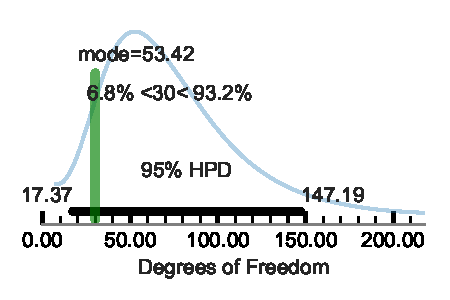
\includegraphics[width=0.5\textwidth]{./hari-code/robust_normality.pdf}
    \caption{The posterior distribution for $\nu$, the normality parameter of the $t$-distribution. When $\nu=\infty$ the $t$-distribution is identical to the Normal distribution. The posterior distribution shows a vertical green bar for $\nu=30$, the traditional cut-off condition on degrees of freedom, for using a Normal distribution. The mode $\nu=53.42$, and the posterior probability distribution implies that only about 7\% of the posterior lies to the left of the green line (i.e. $P(\nu \leq 30) \approx 0.07$), implying that the assuming that the likelihood function to be Normally distributed will give similar inference.}
    \label{fig:normality}
\end{figure}

% Having discussed posterior-prediction checks, model convergence, and normality, next, we discuss alternatives to the model.

% \subsection{Alternative Models}
% \label{sub:Alternative Models}

% As a first instance, consider a similar model, except that the scale parameter of the likelihood function is \textit{not nested} like our current model. Instead, we consider the equal variance case, where all the variances are equal (similar to ANOVA), and that the variance is drawn from a uniform distribution. In other words, $\sigma_j = \sigma \sim U(L, H)$, where $L>0$ and where $H$ is a large constant. The main effect of the equal variance assumption is that there is no information sharing among the groups as would be the case when each $\sigma_j$ is drawn from the same distribution, whose parameters have hyper-priors; the latter is our current model.

% The main effect of constraining our simplified model is that we are slightly poorer in predicting the observed data since all the variances are guaranteed by the model to be equal, whereas we can see from~\Cref{fig:traceplot} that the mean scale (or equivalently variance) in the text condition is lower. We are skipping the traceplot and the contrast plots in this case, as they are similar, to~\Cref{fig:traceplot} and~\Cref{fig:robustcontrasts}, except that the effect size for the combined case is slightly lower due to the equal variance assumption. 

% Instead, we compare the two models using WAIC (Widely Applicable Information Criterion), a principled way to compare models when they have identical likelihood functions~\parencite{Gelman2014a}. WAIC uses the predictive loss to compare two models with different parameters. First, WAIC computes the average log likelihood of each training data point (over the posterior distribution) less the variance of the log likelihood for the same data point; and then it computes the sum over all data points. That is, WAIC for a model: 

% \begin{equation*}
%     \mathrm{WAIC} = -2 \left (\sum_i^N \log \mathrm{Pr}(y_i) - V(y_i) \right) 
% \end{equation*}

% where, $N$ is the total number of training points, $y_i$ is the observation, $\mathrm{Pr}(y_i)$ is the averaged data likelihood over the posterior, and where $V(y_i)$ is the variance of the data likelihood over the posterior. When we compare the two models, one with unequal variances, and one with equal variances. We show our results in~\Cref{tab:WAIC comparison}:

% \npdecimalsign{.}
% \nprounddigits{2}

% \begin{table}[htb]%\footnotesize
%     \centering
%         \caption{WAIC comparison between the model with equal variances against the case when the variances are not constrained to be equal (i.e. we use a hierarchical model). Both cases assume the Student-$t$ likelihood function, the function used in this paper. The columns show respectively, WAIC, pWAIC (the effective number of parameters; also: $\mathrm{pWAIC}=\sum_i V(y_i)$), dWAIC (the difference between the WAIC scores of the other models with the best model), weight (the relative probability that the model explains the data) SE, the standard error of the WAIC estimate, dSE is the standard error of the difference of the current model against the top model. The table shows that the hierarchical model with unequal variances better explains the observations. }\label{tab:WAIC comparison}
%         \begin{tabular}{rcccccc} \toprule
%             Model & WAIC & pWAIC & dWAIC & weight & SE & dSE \\ \midrule
%              Unconstrained variances, hierarchical    & 1102.48    & 3.95 &     0.00 &     1.00 &     14.61 &     0.00    \\
%             Constrained, equal variances & 1104.17 & 3.42 & 1.69 & 0.00 & 14.25 & 1.54        \\ \bottomrule
%         \end{tabular}
    
%     \end{table}

% The results in~\Cref{tab:WAIC comparison} say that model with the unconstrained variances is better at explaining the data than the model with constrained variances; the relative probability that the hierarchical model with unconstrained variances better explains the observation is 1.0 (refer to the weight column in~\Cref{tab:WAIC comparison})

% How useful was the choice of the Student-t drawing distribution~\Cref{eq:bayesian formulation}, instead of assuming that the outcomes are drawn from a Normal distribution? Our analysis of the posterior distribution of the degrees of freedom parameter $\nu$ shows that there is only a small probability ($P(\nu \leq 30) \approx 0.07$) that $\nu \leq 30$. Thus, we may use the Normal likelihood function, without meaningfully affecting the conclusions. Indeed, in our experiments, when we do model the observations with a Normal likelihood, assume equal variances, we find no meaningful differences in the contrasts or the effect sizes, with the Student-$t$ model with equal variances (results omitted due to space constraints).

% Since the charitable donations are bounded to lie between \$0.0 and \$5.0, might we benefit from using bounded likelihood functions like the Beta distribution $Y \sim Beta(\alpha_j, \beta_j)$ to represent the charitable donations $Y_j$ under the different conditions $j$? While a $Beta(\alpha, \beta)$ distribution lies between $[0,1]$, we can scale down the contributions to lie in $[0,1]$ to use with the $Beta(\alpha, \beta)$ distribution. But notice from~\Cref{fig:contributions across conditions} that in each experimental condition, there is a central lobe, and heavy tails at each extreme, notably at \$0.0 and at \$5.0. 

% Our view of models motivated by~\textcite{McElreath2015} is that they represent an \textit{epistemological} claim, not an \textit{ontological} claim (i.e. a physical assumption about the world). Since our goal is to understand the average tendency to give to charity under the different conditions, and not to make predictions (as might be the case if we were trying to model donation with age as a predictor), the fact that the $t$-distribution is not bounded is less relevant here. 



\textcolor{red}{Our posterior predictive check shows that the $t$-distribution models well the heavy tails, and shows that the variances for the comic conditions are different from the text condition. Furthermore, the comparison between the hierarchical model with unconstrained variances and the model with equal variances shows that the hierarchical model is better at explaining the observations. We discuss posterior prediction checks (\Cref{sub:Posterior Predictive Check}) and alternative models (\Cref{sub:Alternative Models}) in detail in the Appendix. }

To summarize, we discussed transparency and utility in small-$n$ studies as motivation for our use of Bayesian modeling. The model shows good convergence with the Gelman-Rubin statistic $\hat{R}$ was virtually identical to 1.0 for all parameters; the effective sample size was greater than 10,000 for all parameters. The modal value of $\nu$, the degrees of freedom parameter was around 53, suggesting that we could also use the Normal likelihood function. 
